\documentclass[11pt]{article}

\usepackage{thumbpdf, amssymb, amsmath, amsthm, microtype,
	    graphicx, verbatim, listings, color, fancybox}
\usepackage[pdftex]{hyperref}
\usepackage[table]{xcolor}
\usepackage[margin=1in]{geometry}
\usepackage{multicol,multirow}
\usepackage{pseudocode}
\usepackage{subfig}
\usepackage{mysty}
\usepackage{multicol,multirow}
\usepackage{subfig}
\usepackage{dcolumn}
\usepackage{fullpage}
\usepackage{palatino}
\usepackage{bbm}
\usepackage{url}
\usepackage{verbatim}
\usepackage{fancybox, fancyvrb}
\usepackage{listings}
\usepackage{color}

\usepackage{algorithm}
\usepackage{algpseudocode}
\usepackage{algorithmicx}

\begin{document}
\begin{titlepage}

\thispagestyle{empty}
\begin{center}
\vspace*{5em}

{\LARGE \bf Large Substitution Boxes \\with Efficient Combinational Implementations}
\vspace*{2em}

{\Large Christopher A. Wood}
\vspace*{.5em}

{\small Department of Computer Science\\
  Rochester Institute of Technology\\
  Rochester, NY 14623 USA\\
  {\tt caw4567@cs.rit.edu }}

\vspace*{3em}

{\large \it Masters Thesis}

\vspace*{3em}

{\large
\renewcommand{\arraystretch}{2}
\begin{tabular}{ l c r }
  Chair: & {\large Professor Stanis{\l}aw P. Radziszowski} & {\tt spr@cs.rit.edu}\\[1ex]
  \multicolumn{3}{ c }{\noindent\rule{8cm}{0.4pt}}\\
  Reader: & Professor Marcin Lukowiak & {\tt mxleec@rit.edu}\\[1ex]
  \multicolumn{3}{ c }{\noindent\rule{8cm}{0.4pt}}\\
  Observer: & Professor Alan Kaminsky & {\tt ark@cs.rit.edu}\\[1ex]
  \multicolumn{3}{ c }{\noindent\rule{8cm}{0.4pt}}\\
  Observer: & Dr. Michael Kurdziel & {\tt mkurdzie@harris.com}\\[1ex]
  \multicolumn{3}{ c }{\noindent\rule{8cm}{0.4pt}}
\end{tabular}
}

\vspace*{3em}

{\large \today}

\end{center}

\vfill

% \begin{abstract}
% Substitution-permutation network (SPN) designs are very popular constructions for 
% symmetric-key cryptographic primitives. The Advanced Encryption Standard is one 
% prime example of an SPN block cipher that adheres to this design strategy. The substitution
% step, often referred to as the S-box, is typically the only nonlinear component
% of such designs that help realize Claude Shannon's principle of confusion - increasing
% the complexity of the relationship between the secret key and the input plaintext. 
% As a result, much research has been devoted to improving the cryptographic strength and implementation
% efficiency of S-boxes so as to prohibit cryptanalysis attacks that exploit
% weak constructions and enable fast and area-efficient hardware implementations on 
% a variety of platforms. Most S-boxes in the literature are bijective functions that have
% $4$ or $8$ bit inputs. In this work, we explore the cryptographic properties and implementation
% options of $16$ bit S-boxes in hopes of stimulating a new perspective of 
% cryptographic research. We study these S-boxes in the context of Boolean functions 
% to determine their strength and present low-area combinational hardware implementations
% for each candidate S-box.
% \end{abstract}

\end{titlepage}

\tableofcontents

\newpage
\section{Problem Statement}
The cryptographic strength of symmetric-key cryptosystems is traditionally based on 
Claude Shannon's properties of confusion and diffusion \cite{Shannon}. 
Confusion can be defined as the complexity of the relationship between the secret key and 
ciphertext, and diffusion can be defined as the degree to which the influence of 
a single input plaintext bit is spread throughout the resulting ciphertext.
Substitution-permutation networks (SPNs) are natural constructions for symmetric-key
cryptosystems that realize confusion and diffusion through substitution and
permutation operations, respectively \cite{Stinson}. 

As the only nonlinear operation in SPNs, the substitution step, 
more commonly referred to as an S(ubstitution)-box, is critically important
in the construction of cryptographically strong block ciphers that are resilient to
common attacks, including linear and differential cryptanalysis, as well as algebraic 
attacks. Furthermore, as these cryptanalysis efforts have evolved over the past 
few decades, and with the selection of the Advanced Encryption 
Standard (AES) symmetric-key block cipher, the construction 
of cryptographically strong S-boxes with efficient
hardware and software implementations in these 
cryptosystems has become a topic of critical research. 

An S-box mapping can be defined as a function $F : GF(2^n) \to GF(2^m)$. To measure
the cryptographic strength of these functions it is common to represent them as vectorial Boolean functions,
where $F(x) = (f_1(x), \dots, f_m(x))$ and $f_i : GF(2^n) \to GF(2)$, for all $1 \leq i \leq m$. Such a representation
enables one to measure its nonlinearity (i.e. measure of distance from affine functions), algebraic
immunity (i.e. difficulty measure of annihilator-based algebraic attacks), resiliency (i.e. balancedness 
and correlation immunity between input and output of the function), and differential uniformity (i.e.
difficulty measure of differential cryptanalysis). 

Practical S-boxes must also be efficiently computable. For this reason, they are typically defined as functions
over finite fields $GF(2^k)$, where $2 | k$. For example, the Rijndael S-box 
is defined as the function $F : GF(2^8) \to GF(2^8)$, $F(a) = Ba^{-1} \oplus c$, where $B$ and
$c$ are a constant $8 \times 8$ matrix and $8$-dimensional vector over $GF(2)$ \cite{Daemen02-1}. If we represent an
input element $a$ and output element $b$ as $a_7a_6a_5a_4a_3a_2a_1a_0$ and 
$b_7b_6b_5b_4b_3b_2b_1b_0$, respectively, where $a_i,b_i \in GF(2)$ for for all 
$0 \leq i \leq 7$, then the S-box $F$ can be defined as:
\begin{align*}
\begin{bmatrix} b_7 \\ b_6 \\ b_5 \\ b_4 \\ b_3 \\ b_2 \\ b_1 \\ b_0 \end{bmatrix} = 
\begin{bmatrix} 
1 & 1 & 1 & 1 & 1 & 0 & 0 & 0 \\
1 & 1 & 1 & 1 & 1 & 0 & 0 & 0 \\
1 & 1 & 1 & 1 & 1 & 0 & 0 & 0 \\
1 & 1 & 1 & 1 & 1 & 0 & 0 & 0 \\
1 & 1 & 1 & 1 & 1 & 0 & 0 & 0 \\
1 & 1 & 1 & 1 & 1 & 0 & 0 & 0 \\
1 & 1 & 1 & 1 & 1 & 0 & 0 & 0 \\ 
1 & 1 & 1 & 1 & 1 & 0 & 0 & 0 \end{bmatrix} \begin{bmatrix} a_7 \\ a_6 \\ a_5 \\ a_4 \\ a_3 \\ a_2 \\ a_1 \\ a_0 \end{bmatrix}^{-1} \oplus
\begin{bmatrix}
c_7 \\ c_6 \\ c_5 \\ c_4 \\ c_3 \\ c_2 \\ c_1 \\ c_0
\end{bmatrix}
\end{align*}
With only $2^8$ elements in $GF(2^8)$, it is possible to tabulate and store
all values $b = F(a)$ for all $a \in GF(2^8)$. With such a lookup table (LUT) data structure, the SubByte
step in the Rijndael algorithm can be computed with a single index into this table. 
There are however some critical flaws with this approach in practical implementations
of the Rijndael algorithm.

First, this implementation strategy is susceptible to cache-timing 
side-channel attacks on systems where the CPU cache size is too small to store the 
entire Rijndael state and S-box LUT. On such systems, it is possible to conduct 
a chosen-plaintext attack requiring anywhere from 
$2^{13}$ to $2^{20}$ samples to perform a full key recovery \cite{Bonneau06-1}. The number of
samples required for this attack is highly dependent on the system properties
and the accuracy of the timing mechanisms available to the attacker. These attacks
are based on timing anomalies that result from cache-collisions (cache hits) 
that occur when performing table lookups at runtime. More specifically, it is possible
to relate bits of the input (or output) to bits of the key that are satisfied
when timing deviations occur. By exploiting this relationship it is possible
to deduce parts of the key until the it can eventually be fully recovered 
or the remaining key space is small enough to perform an exhaustive search. 

Another problem with LUT-based implementations of the S-box is that they require
$2$Kb of memory. In resource constrained systems, 
such as VLSI circuits and embedded platforms, such memory resources
are not readily available. 

Clearly, constant-time S-box mappings with small memory footprints, which
can be achieved at runtime with online calculations in software or combinational logic 
in hardware, are ideal for secure and efficient implementations
of the block ciphers with S-boxes similar to Rijndael. 
Hardware optimization efforts are traditionally focused on
the multiplicative inverse calculation in the S-box, since this is the 
most computationally expensive procedure. 
To date, the most effective technique for minimizing the circuitry required
for the multiplicative inverse calculation is to use composite field
arithmetic to replace the inverse calculation of $a \in GF(2^8)$ with
a series of multiplication, squaring, addition, and an inverse operation
on elements $b,c \in GF(2^4)$. Similar decomposition strategies
can be implemented and optimized in software to yield efficient and 
near constant-time S-box calculations in memory-constrained systems.

The problem of optimizing hardware and software implementations of S-boxes has been 
studied in the literature for more than a decade \cite{Satoh01-1, Mentens05-1, Canright05-1, Boyar12-1}.
Furthermore, with the selection of the Advanced Encryption Standard,
all of this research has been focused on 8-bit S-boxes (i.e. $F : GF(2^8) \to GF(2^8)$).
To our knowledge, there has not been any work that studies the strength and
implementation efficiency (in terms of software throughput and hardware area) of higher order
S-boxes. Therefore, in this thesis, we break away from tradition and focus our 
attention on $16$-bit S-boxes. The problem is to study these S-boxes
in the context of Boolean functions to determine their strength, and for each ideal candidate
S-box, attempt to find optimized hardware and software implementations through 
composite field arithmetic with polynomial bases. Time permitting, we may also explore the 
efficacy of normal and mixed basis decomposition strategies for optimizing the S-box calculations.


\section{Cryptographic Strength of S-Boxes}
The cryptographic strength of S-boxes is often measured using Boolean functions. 
A Boolean function is a function $f : \mathbb{F}_2^n \to \mathbb{F}_2 : GF(2^n) \to GF(2)$ \cite{Cusik09-1}.
For convenience, let $\Omega_n$ be the set of all Boolean functions on $n$ variables. Clearly,
we have that $|\Omega_n| = 2^{2^{n}}$. For all Boolean functions $f \in \Omega_n$ there exists a
unique truth table (TT) or Algebraic Normal Form (ANF) representation. The TT for a Boolean function
$f$ is simply the vector $(f(\bar{0}), \dots, f(\bar{1}))$, where each element corresponds to an element in $GF(2)$. 
The TT representation of Boolean functions offers a simple way to measure the distance between two
Boolean functions $f$ and $g$, since we can simply compute the Hamming distance between them.

Alternatively, we can represent Boolean functions as polynomials in $\mathbb{F}_2[x_0,\dots,x_{n-1}]/(x_0^2 - x_0,\dots,x_{n-1}^2 - x_{n-1})$,
which corresponds to their ANF representation. The process of translating a Boolean function $f$ to its ANF representation
is called the algebraic normal transform, and is defined as follows:
\begin{align*}
f(\bar{x}) = \sum_{i = (i_0,\dots,i_n) \in \mathbb{F}_2^n}a_ix_0^{i_0}x_1^{i_1}\dotsb x_{n-1}^{i_{n-1}} (\text{mod 2}),
%f(\bar{x}) = \bigoplus_{a_0,\dots,a_{n-1}} h(a_0,\dots,a_{n-1})x_0^{a_0} \dots x_{n-1}^{a_{n-1}} = \bigoplus_{\bar{a} \in GF(2^n)} h(\bar{a})\bar{x}^{\bar{a}}
\end{align*}
where $a_i \in \mathbb{F}_2$. S-boxes of the form $F : GF(2^n) \to GF(2^m)$ are unique Boolean functions in that they combine 
the output of $m$ individual Boolean functions in its output. In other words, they 
can be represented as a vector of $m$ Boolean functions $f_i, 1 \leq i \leq m$, that share the same
$n$ input bits, denoted as:
\begin{align*}
f_1(x_1,\dots,x_n) \\
f_2(x_1,\dots,x_n) \\
\vdots \\
f_{m-1}(x_1,\dots,x_n) \\
f_m(x_1,\dots,x_n)
\end{align*}
Based on this definition, we let $F(x) = (f_1(x),\dots,f_m(x))$. Boolean functions of this
type are called vectorial Boolean functions, and we denote them as $F : GF(2^n) \to GF(2)^m$
or $(n,m)$ S-boxes.

Cryptographically significant properties such as nonlinearity, resiliency, and algebraic immunity 
can be measured for a given Boolean function. These measurements are indications of the 
S-boxes susceptibility to linear cryptanalysis, statistical correlation, and algebraic attacks.
Another important property for these S-boxes is differential uniformity, first popularized in
terms of S-boxes by Nyberg in \cite{Nyberg94-1}. It is critically important to examine all
such measurements in the study and development of cryptographically strong S-boxes.

% Another common means of generating the ANF 
% representation is to construct the polynomial which consists of the sum of the polynomial
% $(a_0 \oplus a_0 \oplus 1)\dots(x_{n-1} \oplus a_{n-1} \oplus 1)$ for all $\bar{a} \in GF(2^n)$ such that $f(\bar{a}) = 1$. 
% This definition can be described as the following.
% \begin{align*}
% ANF(\bar{x}) = &  a_0 \oplus \\
% &  a_1x_1 \oplus ... \oplus a_{n}x_{n} \oplus \\
% &  a_{1,2}x_1x_2\oplus ... \oplus a_{n-1, n}x_{n-1}x_n \oplus \\
% &  ... \\
% &  a_{1,2,...,n}x_{1}...x_{n}
% \end{align*}

\subsection{Nonlinearity}
Since Boolean functions are natural representations for S-boxes, the measure of nonlinearity becomes
fundamental in the assessment of the cryptographic strength of S-boxes. For a Boolean function $f$,
we define the nonlinearity $\nl$ as follows:
\begin{align*}
\nl = \min_{\phi \in \mathcal{A}_n} d(f, \phi),
\end{align*}
where $\mathcal{A}_n$ is the set of all Boolean affine functions on $n$ variables, 
and $d(f, g) = wt(f \oplus g)$ (i.e. the Hamming distance between two functions $f$ and $g$) \cite{Cusik09-1}. 
Cryptographically strong S-boxes have high measures of nonlinearity, meaning that
it is increasingly difficult to approximate them using linear affine functions.
Subsequently, high measures of nonlinearity help hinder linear cryptanalysis attacks. 

\subsection{Resiliency}
Resiliency combines the measurements of balancedness and correlation immunity. 
Balancedness is a simple property of Boolean functions that captures the distribution of their output.
In particular, a Boolean function is balanced if its (Hamming) weight is $2^{n - 1}$. 
A Boolean function $f$ on $n$ variables is said to have a correlation immunity 
of order $t$, $1 \leq t \leq n$, if the output is statistically independent for any fixed subset of at most $t$ 
variables. In other words, given $f(\bar{x})$, the probability that $t$ fixed input variables have 
any set of values is always $2^{-t}$. Correlation immunity is an important property of 
cryptosystems with the advent of correlation attacks on stream ciphers \cite{Canteaut05-1}.
A higher correlation immunity indicates a lower susceptibility to such attacks.

\subsection{Algebraic Immunity}
This metric is used to determine a Boolean functions resilience to attacks
based on annihilators \cite{Cusik09-1}. Formally, an annihilator of a Boolean 
function $f$ is another a Boolean function $g$ such that $f \oplus g = 0$. 
Using low-degree annihilators it is sometimes possible to reduce the degree
of a Boolean function to a small enough value such that the system of 
equations relating the Boolean function and state or key bits of a cryptosystem
can be solved in a reasonable amount of time \cite{Frederik04-1}. 

\subsection{Differential Uniformity}
Differential uniformity relates to the S-boxes resistance to differential cryptanalysis
attacks. First introduced in 1994 by Nyberg \cite{Nyberg94-1}, we say that
an S-box $F : GF(2^n) \to GF(2^m)$ is $\delta$-differentially uniform if for all $\alpha \in GF(2^n)$
and $\beta \in GF(2^m)$ we have
\begin{align*}
|\{x \in GF(2^n) | F(x + \alpha) = \beta\}| \leq \delta.
\end{align*}
Differential cryptanalysis exploits the lack of uniformity in the nonlinear S-box
step of SPN block ciphers. Cryptographically strong S-boxes have low values for
$\delta$, as this means the output of $F$ is relatively uniform and the frequency of a 
single output value cannot be easily exploited for an attack. 
Differential uniformity was first studied in the context of the Data Encryption
Standard, and it was proven in \cite{Nyberg94-1} that if the round functions of
Feistel-based ciphers similar to DES are $\delta$-differentially uniform, then 
the average probability to obtain a non-zero output for input $x + \alpha$, for
all $x, \alpha \in GF(2^n)$, after a fixed number of rounds is bounded by $2(\frac{\delta}{2^n})^2$.

S-boxes of the form $F(x) : x^{-1}$ were shown to be $4$-differentially uniform 
with a $\nl$ lower bound of $2^{n-1} - 2^{\frac{n}{2}}$ in \cite{Nyberg94-1}.
Similarly, S-boxes of the form $F(x) = x^{2^{k} + 1}$ are $2$-differentially uniform
with a $\nl$ equal to precisely $2^{n-1} - 2^{\frac{n-1}{2}}$. With the selection
of Rijndael as the AES in 2001 \cite{Daemen02-1}, S-boxes of the form $F(x) : x^{-1}$
became the primary subject of study in the literature. 

% TODO: normal basis implementation for efficient squaring of this power mapping? YES PLEASE!

\subsection{Construction Techniques}
Constructing cryptographically significant Boolean functions is a well-studied problem
in the literature. For the purposes of this work, we restrict ourselves to a 
single class of Boolean function constructions belonging to the Maiorana-McFarland
class of functions, which are used to construct bent functions \cite{Gupta05-1, Gupta02-1}. 
These construction techniques can be used to build $(n,m,t)$ resilient S-boxes with
degree $d > m$. Efficient software implementations of similar functions are
presented in \cite{Gupta02-1}. Furthermore, as Boolean functions, the output of these
constructions can be directly mapped to combinational logic and implemented in hardware. 

%http://arxiv.org/pdf/1003.3492v1.pdf

\section{Techniques for Efficient Implementations}
Computing the multiplicative inverse of elements in $GF(2^k), k = nm,$ is a long-studied
problem dating back to the early 1990s \cite{Brunner93-1}. At the time, computing
inverses using Fermat's theorem or the Extended Euclidean algorithm were popular 
techniques. Modern approaches for minimizing the circuit complexity of the multiplicative inverse step
rely on composite field arithmetic to reduce the operations
to elements in smaller fields. Such decompositions often rely on a change in basis between
two fields, where the change is between polynomial and normal bases.
We discuss recent work of both schemes in the following sections.

\subsection{Composite Field Representations for Inverses}
A \emph{composite field} is a pair $\{GF(2^n), Q(y) = y^n + \sum_{i=0}^{n-1}q_iy^i, q_i \in GF(2)\}$ and
$\{GF((2^n)^m), P(x) = x^m + \sum_{i=0}^{m-1}p_ix^i, p_i \in GF(2^n)\}$ where $GF(2^n)$ 
is constructed from $GF(2)$ by $Q(y)$, and $GF((2^n)^m)$ is constructed from 
$GF(2^n)$ by $P(x)$. We state that $GF((2^n)^m)$ is a degree $m$ extension of $GF(2^n)$.
This form of extension means that the coefficients of the polynomials in $GF((2^n)^m)$
are themselves elements of $GF(2^n)$. 

Using composite field arithmetic, it is possible to reduce the multiplicative
inverse calculation of elements $a \in GF(2^k)$ to calculations in $GF((2^n)^m)$.
In particular, given a composite field $GF((2^n)^m)$, where $m = 2$ and $P(x) = x^2 + Ax + B$,
there exists a decomposition from $GF(2^k)$ to $GF((2^n)^m)$. With such a
decomposition, we can now compute $a^{-1}$ as follows:
\begin{align}
a^{-1} = (bx + c)^{-1} = b(b^2B + bcA + c^2)x^{-1} + (c + bA)(b^2B + bcA + c^2)^{-1},
\end{align}
\begin{figure}[ht!]
\begin{center}
	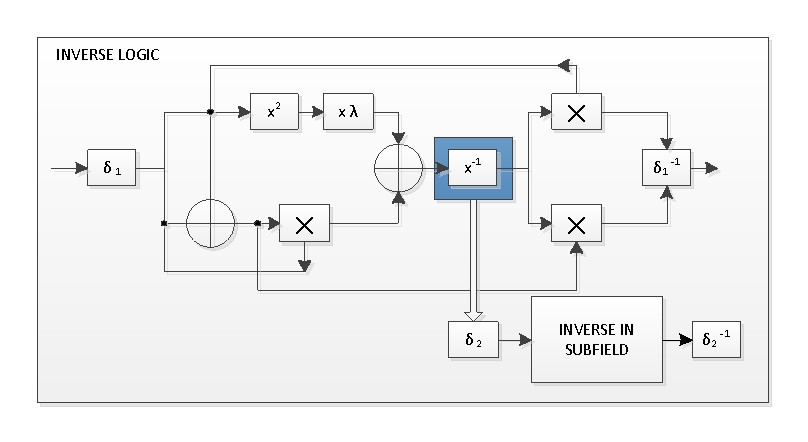
\includegraphics{images/composite_field_inverter.pdf}
\end{center}
\caption{Multiplicative inverse calculation using composite field decomposition. The blocks $\delta_1$ and
$\delta_1^{-1}$ are constant multiplications with the basis transformation matrices from $GF(2^k)$ to
$GF((2^n)^m)$, respectively. }
\label{fig:compositeFieldInverse}
\end{figure}
The circuitry required to implement this calculation is shown in Figure \ref{fig:compositeFieldInverse}. 
Since $b, c, B, A \in GF(2^n)$, we can recursively decompose the inverse of $(b^2B + bcA + c^2)$ into
elements of the field $GF(2^{n/2})$ (assuming $GF(2^n)$ can be represented as a degree $2$ extension
of the field $GF(2^{n/2})$). Such designs are referred to as tower field decompositions. Satoh et al.
explored all tower field decompositions for $GF(2^8)$ in \cite{Satoh01-1}. The field extensions they 
used are shown below, where $\phi \in GF(2^2)$ and $\lambda \in GF((2^2)^2)$ are chosen such that $P(x)$
is irreducible over their respective extension fields.
\begin{align*}
GF(2) \to GF(2^2)\text{ , }& P(x) = x^2 + x + 1 \\
GF(2^2) \to GF((2^2)^2)\text{ , }& P(x) = x^2 + x + \phi \\
GF((2^2)^2) \to GF(((2^2)^2)^2)\text{ , }& P(x) = x^2 + x + \lambda 
\end{align*}
To convert between elements in $GF(2^k)$ and $GF((2^n)^m)$ represented in 
a polynomial basis, where $k = nm$, it is necessary to find a mapping between 
these two fields such that additive and multiplicative homomorphism is maintained. 
A polynomial basis for a field $GF(2^k)$ defined by a primitive irreducible polynomial $P(x)$
and primitive element $x$ is the set $\{x^{k-1}, \dots,x^2,x,1\}$. Each element
in this basis is linearly independent from all others, so it is possible to represent every element
in the field using this basis. In addition, the basis element $x$ can 
be used to generate every element in the field $GF(2^k)$ as $\{0, 1, x,\dots, x^{p^{k} - 2}\}$.
By finding two primitive elements $\alpha \in GF(2^k)$ and $\beta \in GF((2^n)^m)$, 
the mapping $\alpha^i \to \beta^i, 0 \leq i \leq 2^k - 1$ can then be defined 
by mapping the basis $\alpha$ of $GF(2^k)$ to the basis $\beta$ of $GF((2^n)^m)$.
The result is a binary $k \times k$ matrix \textbf{T} such that \textbf{T}$\alpha^i = \beta^i$.
This matrix can be defined by \textbf{T}$ = [(\beta^0)^T, (\beta^1)^T,\dots,(\beta^{k-1})^T]$.
The transformation matrix \textbf{T} and its inverse \textbf{T}$^{-1}$ used by Satoh et al.
are shown below.
\begin{align*}
	\text{\textbf{T}} =  \left( \begin{array}{cccccccc}
1 & 1 & 0 & 0 & 0 & 0 & 1 & 0 \\
0 & 1 & 0 & 0 & 1 & 0 & 1 & 0 \\
0 & 1 & 1 & 1 & 1 & 0 & 0 & 1 \\
0 & 1 & 1 & 0 & 0 & 0 & 1 & 1 \\
0 & 1 & 1 & 1 & 0 & 1 & 0 & 1 \\
0 & 0 & 1 & 1 & 0 & 1 & 0 & 1 \\
0 & 1 & 1 & 1 & 1 & 0 & 1 & 1 \\
0 & 0 & 0 & 0 & 0 & 1 & 0 & 1 \end{array} \right) \hspace{2em} \text{\textbf{T}}^{-1} = 
\left( \begin{array}{cccccccc}
1 & 0 & 1 & 0 & 1 & 1 & 1 & 0 \\
0 & 0 & 0 & 0 & 1 & 1 & 0 & 0 \\
0 & 1 & 1 & 1 & 1 & 0 & 0 & 1 \\
0 & 1 & 1 & 1 & 1 & 1 & 0 & 0 \\
0 & 1 & 1 & 0 & 1 & 1 & 1 & 0 \\
0 & 1 & 0 & 0 & 0 & 1 & 1 & 0 \\
0 & 0 & 1 & 0 & 0 & 0 & 1 & 0 \\
0 & 1 & 0 & 0 & 0 & 1 & 1 & 1 \end{array} \right)
\end{align*}
The complexity of the S-box calculation is based on the transformation matrix used to map every element
$\alpha \in GF(2^k)$ to an element $\beta \in GF((2^n)^m)$, as well as the constant multiplication 
operations in the multiplicative inverse block, both of which depend on the choice of
irreducible polynomials for $P(x)$. Rudra et al. \cite{Rudra01-1} present functions for
estimating the gate complexity of an S-box given the field representations. Once optimized solutions for the
gate complexity are found, the Boolean logic for the transformation matrices can be further
simplified using a greedy compression algorithm, as presented in \cite{Morioka99-1}.
Mentens et al. \cite{Mentens05-1} examined the composite field definitions and corresponding
S-box used by Satoh et al. and showed that their results were 5\% away from an optimal solution.
This was determined by choosing a different constant $\lambda = \{1000\}_2$ such that the 
base field multiplication operation in (1) contains one additional XOR gate with the benefit
of reducing the complexity of the transformation matrix \textbf{T} by 5 gates.

\subsection{Normal Basis Transformations}
The normal basis for a finite field $GF(2^k)$ is defined as the set $\{\beta, \beta^2, \beta^{2^2},\dots,\beta^{2^{k-1}}\}$, 
where $\beta \in GF(2^k)$ and all elements in the set are linearly independent. An immediate result of representing
elements using the normal basis of a field is that squaring comes for free in hardware (i.e. it equates to a bit-wise
rotation of the element). For this reason, composite field decompositions using normal bases, rather than polynomial
bases, have been another popular topic of research in the literature \cite{Nikova08-1, Canright05-1}.

When the multiplicative inverse calculation is decomposed into operations on smaller fields
represented in a normal basis, multiplication and inversion in the base field are still the most expensive procedures of the 
entire calculation. With this basis representation, the multiplicative
inverse operation can be expressed in very elegant equations, as shown in \cite{Nikova08-1}. 
For both of these operations, let $ax + b$ and $cx + d$ be two elements in $GF((2^n)^m)$,
and let $\{v,m v^l\}$ be a normal basis of $GF((2^n)^m)$. The product of these
two elements is $ex + f = (ax + b) \times (cx + d)$, where $e = (a + b)(c + d)g + ac, f = (a + b)(c + d)g + bd$ and 
$g = v^2 + v$ (the trace of $v$ over $GF(2^n))$. Similarly, the inverse $(ax + b)^{-1}$ can be defined
as $(cx + d) = (ax + b)^{-1}$, where $c = ((a + b)^2g + ab)^{-1}b$ and $((a + b)^2g + ab)^{-1}a$.
Again, the inverse operation requires one to calculate the inverse of elements over $GF(2^n)$,
and so this process can be repeated recursively. Alternatively, the inverse of elements in $GF(2^n)$ 
may be optimized using Boolean function minimization based on its ANF representation, as is done in \cite{Nikova08-1}. 

%\subsection{Fermat's Theorem for Inverse}
%TODO: inverse and derivation here (and comment about rotation)
%\subsection{Normal Basis}
%TODO: describe how normal basis works and why squaring is free
\section{Proposed Work}
The first part of our research will focus on the cryptographic strength of 
various S-box definitions using analysis methods for Boolean functions. Clearly, exhaustively searching
all $GF(2^{2^{16}})$ S-box definitions is infeasible, so our analysis will be constrained
to S-boxes defined by differentially uniform mappings over Galois fields, such as the
inverse mapping $F(x) = x^{-1}, x \in GF(2^{16})$, and built 
using the Maiorana-McFarland Boolean function construction technique. Time
permitting, we may also explore Boolean function construction techniques targeted towards specific
cryptographic properties, such as resiliency and algebraic immunity. 
The metrics collected for this part of the research include the nonlinearity,
algebraic immunity, resiliency, and differential uniformity of each S-box candidate. 
Some of these metrics can be gathered using third-party software tools like 
SAGE and Mathematica, while others will require custom software to measure. Such
software would be part of the deliverables for this thesis, and it will be used
to weigh the strength and weaknesses of various S-box definitions. 
 
The second thread of our research will be to implement candidate S-boxes in FPGA hardware and generate 
similar equivalent ASIC models. To facilitate the selection of candidate S-boxes, 
we will study the gate-level complexity of ideal S-boxes using various
representations defined by different irreducible polynomials. These implementation techniques will explore the composite field
decomposition techniques using polynomial bases. Time permitting, we will also explore the optimizations
that are possible with normal basis representations of the S-boxes. While mixing these two representations
will likely lead to an improved solution, such work is outside the scope of this thesis. A major outcome
of this thread of research is to determine the implementation differences between FPGA and ASIC platforms
in terms of hardware resource and power consumption. Composite field decompositions do not currently benefit
on FPGA platforms due to the small size of logic required for the functions and the larger LUT blocks. 
It is unclear as to whether or not this problem will be subverted with 16-bit S-boxes, and so we hope 
to address this issue. 

Software versions of these functions will also be implemented to measure the throughput performance
on low-end platforms (e.g. 32-bit PowerPC hardcore processors).
The metrics collected for this part of the research include hardware area (i.e.
FPGA slices and total synthesized logic gates) and throughput (cycles per byte), as well
as the software memory footprint for S-box functions and their throughput (cycles per byte).
These software implementations will be compared against LUT-based implementations in terms of 
memory usage and throughput. 
\input{./metrics}
\input{./evaluation}
\section{Deliverables}
When the proposed work is complete, a written thesis report will be submitted. The report will include all background information needed, including that which has been included in this proposal. All results will be documented. The following utility software will be submitted as part of the deliverables.
\begin{itemize}
	\item Generic Galois field mathematical library that supports field extensions, composite field arithmetic, and finding primitive irreducible polynomials.
	\item Boolean function construction and analysis software.
	\item Field representation optimization library for minimizing the gate-level complexity of mathematical operations.
\end{itemize}
At a minimum, the following S-box implementations will also be submitted with the deliverables.
\begin{itemize}
	\item LUT-based and optimized software implementations of candidate S-boxes for low-end processors.
	\item Traditional (unoptimized) and optimized composite field HDL models for FPGA and ASIC implementations of candidate S-boxes. 
\end{itemize}
Relevant data obtained from experiments, including all Boolean function properties and hardware implementation metrics, will be displayed in 
the most appropriate format. Finally, an appendix will be attached that contains all of the source code implemented for this project.

\subsection{Timeline}
The thesis will be written in parallel with the research. Both stages of the research (cryptographic strength analysis and
implementation optimizations) will overlap, and will not be completed in full until the thesis is finished. The following schedule
depicts the workflow and major milestones for the thesis. 

\begin{center}
\begin{tabular}{ l | p{8cm} }
  Date & Task \\ \hline
  April 8, 2013 & Complete thesis proposal submission \\
  April 12, 2013 & Finish the 8-bit S-box experiment methodology and test framework \\
  April 19, 2013 & Implement software for Boolean function analysis, constructions, and HDL translations \\
  April 26, 2013 & Finish the first candidate $16$-bit S-box model in HDL \\
  May 10, 2013 & Finish and measure the implementation of all candidate $16$-bit S-boxes using only polynomial basis representations \\
  May 31, 2013 & Design an HDL model normal basis representation of an $8$-bit S-box. \\
  Jun 7, 2013 & Finish and measure the hardware implementation of $16$-bit S-boxes built on designs in the literature (tentative). \\
  June 14, 2013 & Finish and measure the software implementations of all candidate S-boxes for low-end platforms. \\
  July 5, 2013 & Finish thesis report \\
  August 5, 2013 & Defend thesis
\end{tabular}
\end{center}

\vspace*{2em}

\begin{thebibliography}{9}

\bibitem{Shannon} Claude E. Shannon. Communication Theory of Secrecy Systems. Bell System Technical Journal 28.4 (1949), 656-715.

\bibitem{Stinson} Douglas Robert Stinson. Cryptography: Theory and Practice. CRC press (2006).

\bibitem{Bonneau06-1} Joseph Bonneau and Ilya Mironov. Cache-Collision Timing Attacks Against AES. Cryptographic Hardware and Embedded Systems-CHES 2006. Springer Berlin Heidelberg (2006), 201-215.

\bibitem{Satoh01-1} Akashi Satoh, Sumio Morioka, Kohji Takano, and Seiji Munetoh. A Compact Rijndael Hardware Architecture with S-box Optimization. Advances in Cryptology—ASIACRYPT 2001. Springer Berlin Heidelberg (2001), 239-254.

\bibitem{Mentens05-1} Nele Mentens, Lejla Batina, Bart Preneel, and Ingrid Verbauwhede. A Systematic Evaluation of Compact Hardware Implementations for the Rijndael S-box. Topics in Cryptology–CT-RSA 2005. Springer Berlin Heidelberg (2005), 323-333.

\bibitem{Canright05-1} David Canright. A Very Compact S-box for AES. Cryptographic Hardware and Embedded Systems - CHES 2005. Springer Berlin Heidelberg (2005), 441-455.

\bibitem{Boyar12-1} Joan Boyar and Ren\'{e} Peralta. A Small Depth-16 Circuit for the AES S-box. Information Security and Privacy Research. Springer Berlin Heidelberg (2012), 287-298.

\bibitem{Brunner93-1} Hannes Brunner, Andreas Curiger, and Max Hofstetter. On Computing Multiplicative Inverses in $GF(2^m)$. IEEE Transactions on Computers, Vol. 42, No. 8, August (1993), 1010-1015.

\bibitem{Paar94} Chirstof Paar. Efficient VLSI Architectures for Bit-Parallel Computations in Galois Fields. PhD Thesis, Institute for Experimental Mathematics, University of Essen, Germany (1994).

\bibitem{Nyberg94-1} Kaisa Nyberg. Differentially Uniform Mappings for Cryptography. Advances in Cryptology - Eurocrypt’93. Springer Berlin Heidelberg (1994).

\bibitem{Cusik09-1} Thomas W. Cusick and Pantelimon St\v{a}nic\v{a}. Cryptographic Boolean Functions and Applications. 
Academic Press (2009).

\bibitem{Canteaut05-1} Anne Canteaut. Fast Correlation Attacks Against Stream Ciphers and Related Open Problems. 
Theory and Practice in Information-Theoretic Security (2005).

\bibitem{Daemen02-1} Joan Daemen and Vincent Rijmen. The design of Rijndael: AES-the advanced encryption standard. Springer (2002).

\bibitem{Gupta05-1} Kishan Chand Gupta and Palash Sarkar. Efficient representation and software implementation of resilient Maiorana-McFarland S-boxes. Information Security Applications. Springer Berlin Heidelberg (2005), 317-331.

\bibitem{Gupta02-1} Kishan Chand Gupta and Palash Sarkar. Improved Construction of Nonlinear Resilient S-boxes. Advances in Cryptology—ASIACRYPT 2002. Springer Berlin Heidelberg (2002), 466-483.

\bibitem{Rudra01-1} Atri Rudra, Pradeep K. Dubey, Charanjit S. Jutla, Vijay Kumar, Josyula R. Rao, and Pankaj Rohatgi. Efficient Rijndael Encryption Implementation with Composite Field Arithmetic. Cryptographic Hardware and Embedded Systems - CHES 2001. Springer Berlin Heidelberg (2001).

\bibitem{Morioka99-1} Sumio Morioka and Yasunao Katayama. Design Methodology for a One-Shot Reed-Solomon Encoder and Decoder. IEEE International Conference on Computer Design - ICCD'99, (1999).

\bibitem{Nikova08-1} Svetla Nikova, Vincent Rijmen, and Martin Schl\H{a}ffer. Using Normal Bases for Compact Hardware Implementations of the AES S-box. Security and Cryptography for Networks. Springer Berlin Heidelberg (2008), 236-245.

\bibitem{Frederik04-1} Frederik Armknecht. On the Existence of Low-Degree Equations for Algebraic Attacks. \emph{State of the Art of Stream Ciphers} (2004), 175-189.

\end{thebibliography}
\end{document}
